\documentclass[border=5pt]{standalone}

\usepackage{tikz}
\usetikzlibrary{arrows, matrix, calc}

\newcommand{\athir}[2]{\displaystyle H^{#1}(B; H^{#2}(F))}


\begin{document}
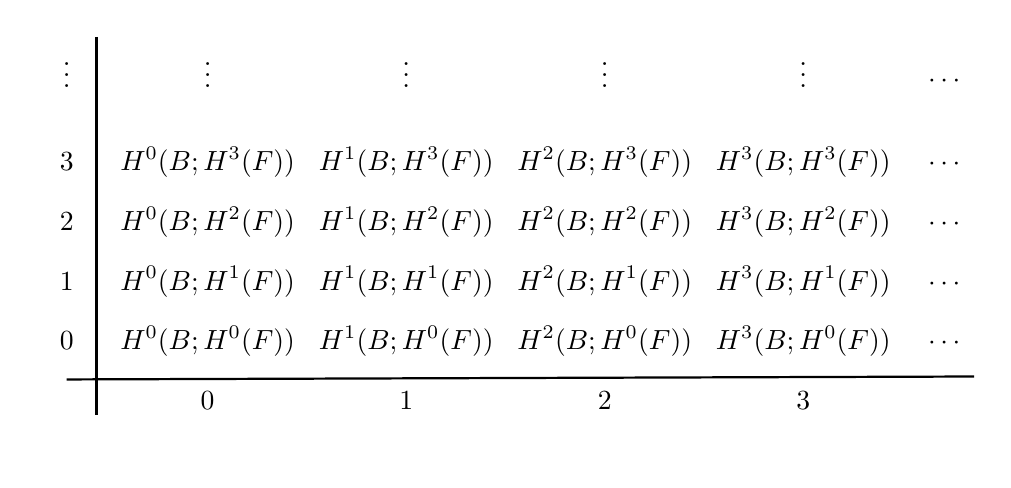
\begin{tikzpicture}
\matrix (m) [matrix of math nodes,
             nodes in empty cells,
             nodes={minimum width=5ex, minimum height=6ex,
                    text depth=1ex,
                    inner sep=0pt, outer sep=0pt,
                    anchor=base},
             column sep=2ex, row sep=2ex]%
{
\vdots  & \vdots       & \vdots       & \vdots & \vdots       & \cdots \\
    [5ex,between origins]
    3 & \athir{0}{3} & \athir{1}{3} & \athir{2}{3} & \athir{3}{3} & \cdots \\
    [3ex,between origins]
    2 & \athir{0}{2} & \athir{1}{2} & \athir{2}{2} & \athir{3}{2} & \cdots \\
    [3ex,between origins]
    1   &   \athir{0}{1} & \athir{1}{1} & \athir{2}{1} & \athir{3}{1} & \cdots \\
    [3ex,between origins]
    0   &   \athir{0}{0} & \athir{1}{0} & \athir{2}{0} & \athir{3}{0} & \cdots \\
    [3ex,between origins]
        &  0           &  1           & 2 &  3         & \strut \\
};
%\draw[-stealth] (m-1-3) -- (m-1-3 -| m-1-2.east);

\draw[thick] (m-1-1.north east) -- (m-6-1.east) ;
\draw[thick] (m-6-1.north) -- ($(m-5-6.east)!0.5!(m-6-6.east)$) ;
\end{tikzpicture}


\end{document}

